% Requirements
% Analysis of requirements
% Discuss the requirements of the project, and what is needed to complete the project.
% Comparison of systems
% For some projects there may be similar existing systems. This would be a good place to identify these, compare them and elicit requirements from them.
% Requirements elicitation
% Perhaps you have conducted some actual research with questionnaires and interviews and such like (having obtained research ethics clearance of course). This would be a good place to discuss this.
% Functional requirements
% A clear statement of functional requirements is the starting point for your design. Without this you will look foolish.
% Non-functional requirements
% Clear statement of non-functional requirements. It may be an idea here to refer back to your earlier LSEPi section as compliance is likely to (and should) be an important aspect here.
\subsubsection{Requirements}
% Establish what quality software means.
% How should I monitor and measure my goals.
% What can I follow as a guide to ensure I am on the right track (e.g. existing tools, gantt charts, etc).
% Use of a widely accepted programming language.
% For the gantt chart instead of displaying tasks on the timeline, put a preliminary task and use the CI pipeline to update the gantt chart with the tasks that are being worked on.

For the development of this project, a multitude of base requirements should be laid out so that project has a structure to follow. These requirements will be used to guide the development of the project and ensure that the project is on track to meet the goals that have been set out.
As the CI pipeline is to be used this will require continuous updating of the "todo" list as the list will change as new features get marked off when started, completed or dropped from the project pipeline as the project progresses (see figure \ref{fig:CodeTodoList}). By having an adaptive todo list it allows for the project to be more flexible and allows for the project to be more easily adapted to changes in requirements, goals or new discoveries that may be made during the development of the project. The downside to such an approach is that it is less structured and so it can be harder to follow and find a set goal. However, it can still be suitable for this project as the goals and features are modular, as will be seen in section \ref{sec:DesignPhilosophy}, how there is no set way to restructure code and so the tool will be updated with new features as they are discovered or needed.
Another major requirement is the analysis of how to measure the current progress of the project through time management. While this is not as easy to do due to the nature of a CI pipeline, it is still important to make assumptions and estimates on how long each task will take to complete and how much of the alloted time should be spent on certain tasks. A project timeline will be used to aid in the time management of the project which will be updated as the project progresses (see figure \ref{fig:ProjectTimelineChart}). It is important to follow this timeline, otherwise if the project time went unmanaged, it may result in incomplete or rushed features that are not up to the standard that is expected Additionally, too much time may be spent on tasks and potentially not leaving enough time for others. A Gantt chart can also be useful as it also shows interdependencies of activities and so delays in some areas may delay the overall project and this can be equally seen when the tasks are updated (see figure \ref{fig:GanttChart}). This can then help identify if other tasks can be completed sooner to avoid delays if changes are required or the overall delay is accepted.

\begin{figure}
    \centering
    \caption{Code TODO List}
    \label{fig:CodeTodoList}
    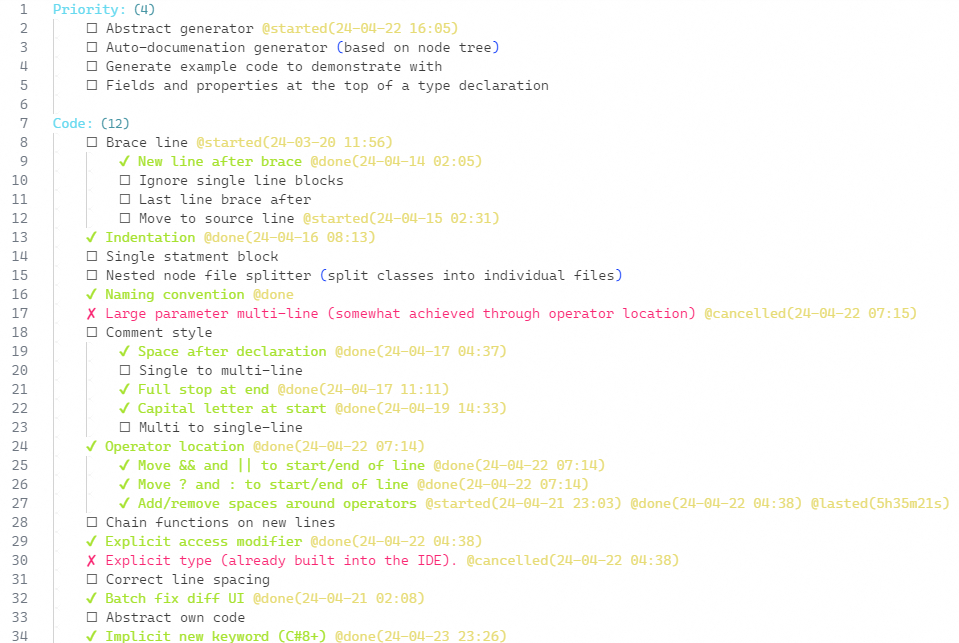
\includegraphics[width=0.7\textheight]{Figures/CodeTodo.png}
\end{figure}

% \newpage
% https://tex.stackexchange.com/questions/144462/latex-figure-or-table-in-a-new-page
% https://tex.stackexchange.com/questions/229440/insert-two-images-as-subfigures-vertically
% MOVED TO APPENDIX
% \begin{figure}
%     \centering
%     \caption{Project Timeline}
%     \label{fig:ProjectTimeline}
%     \begin{subfigure}[t]{0.5\textwidth}
%         \caption{Timeline table}
%         \label{fig:ProjectTimelineChart}
%         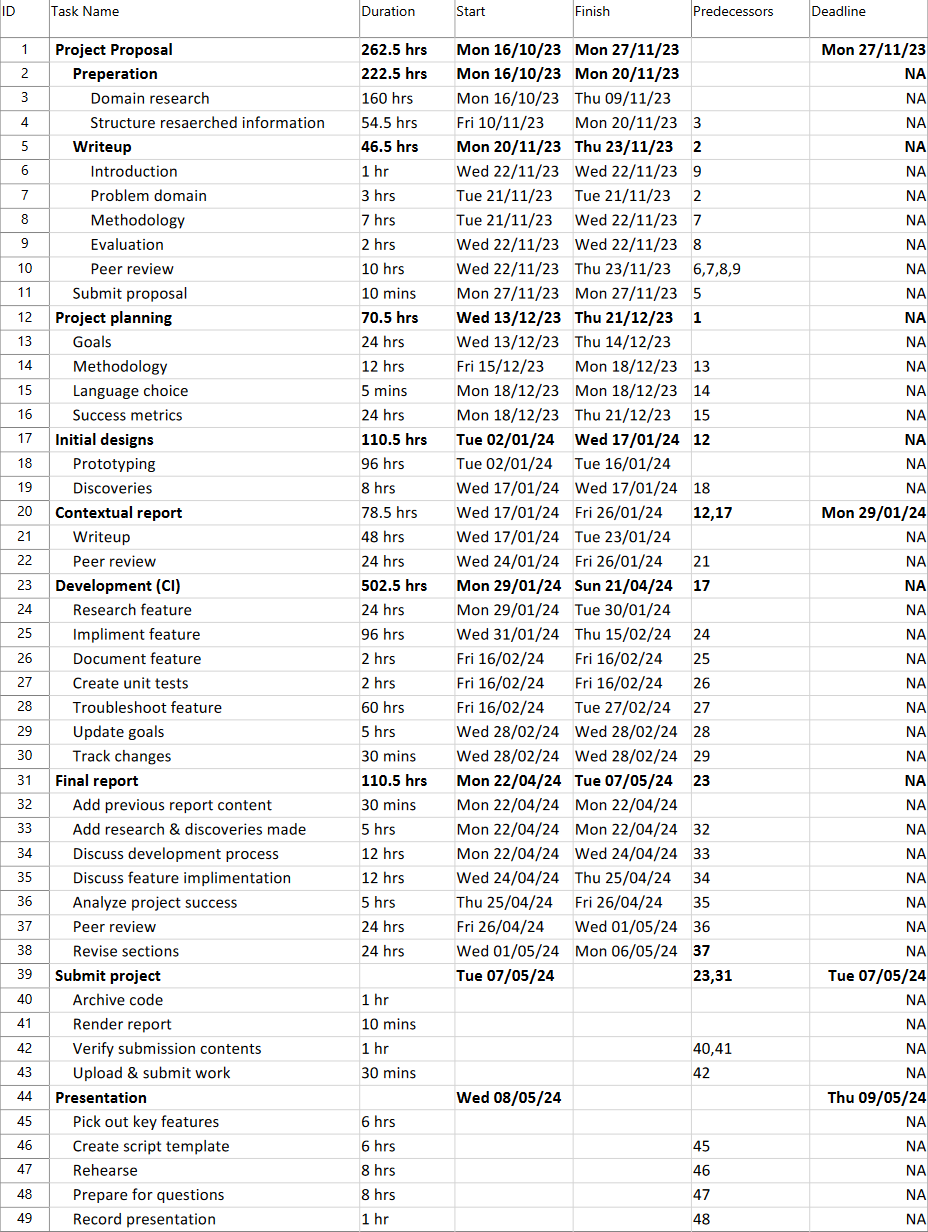
\includegraphics[clip, width=0.5\textheight]{../TimelineChart.png}
%     \end{subfigure}
%     \begin{subfigure}[b]{0.5\textwidth}
%         \caption{Gantt chart}
%         \label{fig:GanttChart}
%         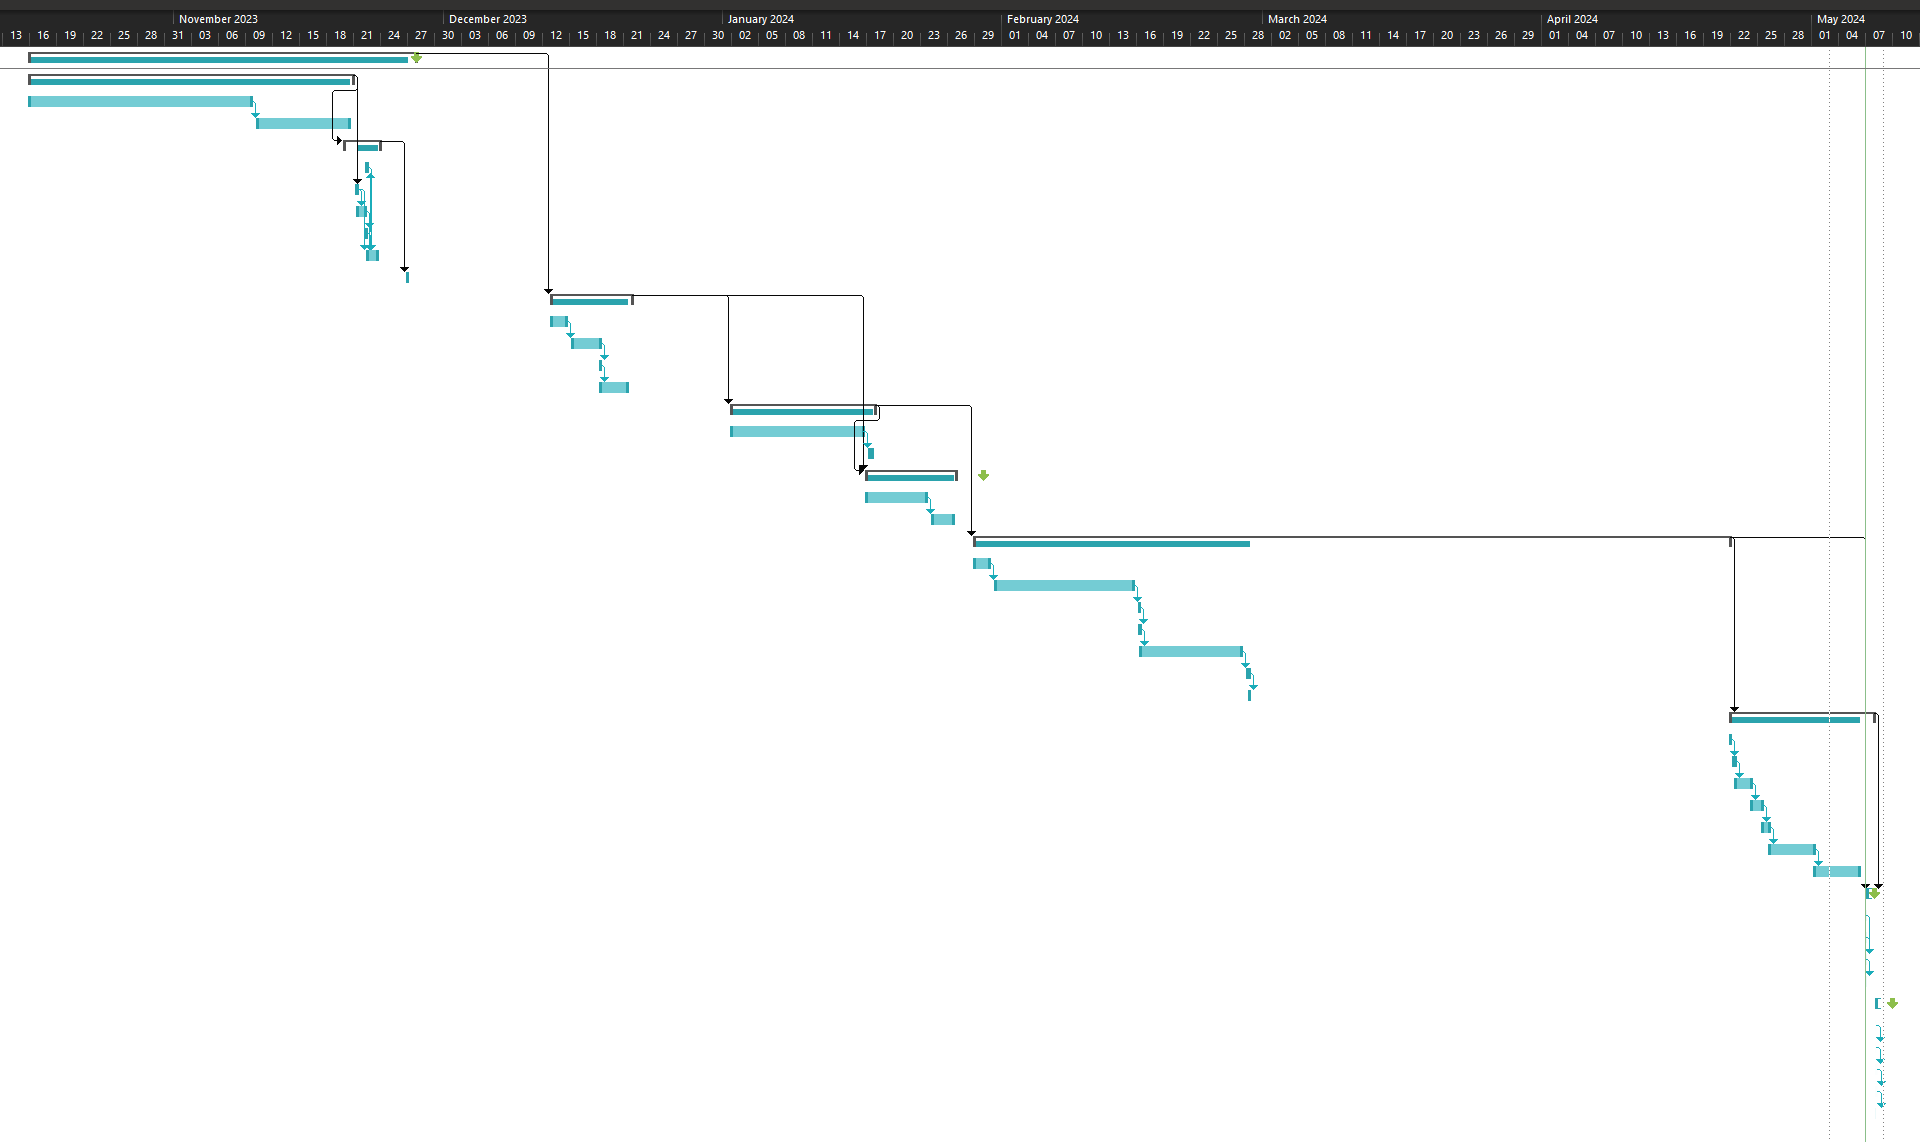
\includegraphics[clip, width=0.5\textheight]{Figures/GanttChart.png}
%     \end{subfigure}
% \end{figure}
